% Fig1.tex -- Fig. 1 of the Information Systems Frontiers version (Springer Nature sn-jnl):
% the pipeline figure redrawn for the 5.15 in text width with 8 pt Arial lettering.
% The numbers are the same as in fig1-pipeline.tex, which make_figures.py writes from the ledger.
% Compile with XeLaTeX (fontspec):  tectonic Fig1.tex   ->  Fig1.pdf
\documentclass[border=1pt]{standalone}
\usepackage{fontspec}
\setmainfont{Arial}\setsansfont{Arial}
\renewcommand{\familydefault}{\sfdefault}
\usepackage{tikz}
\begin{document}
\fontsize{8}{9.6}\selectfont
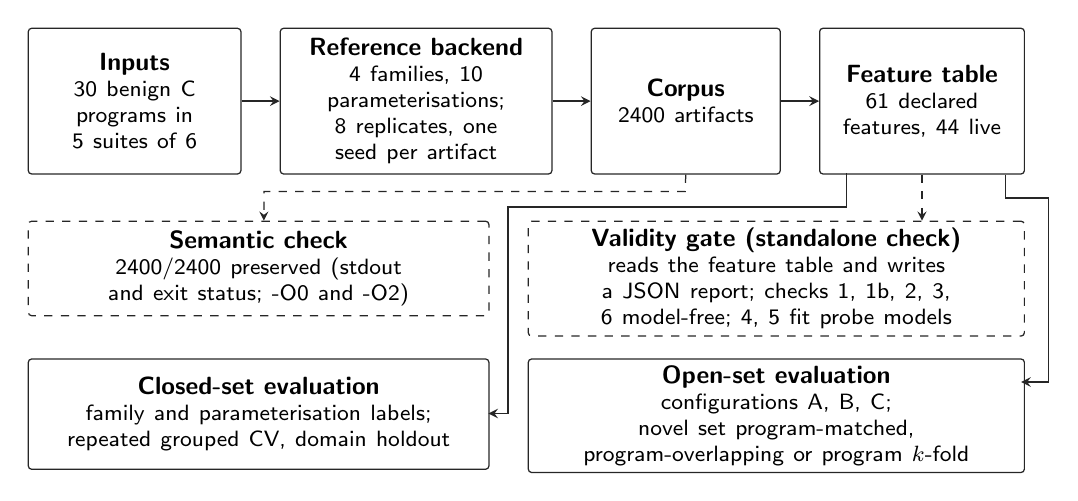
\begin{tikzpicture}[x=1cm,y=1cm,>=stealth,
  stage/.style={draw=black!85,line width=0.45pt,rounded corners=1.2pt,align=center,
                inner xsep=2pt,inner ysep=2.5pt,anchor=north west,
                execute at begin node={\fontsize{8}{9.4}\selectfont\hyphenpenalty=10000\relax}},
  check/.style={stage,dashed},
  flow/.style={->,line width=0.55pt,black!85},
  aux/.style={->,line width=0.45pt,dashed,black!85}]
% row 1: construction
\node[stage,minimum width=2.70cm,text width=2.55cm,minimum height=1.85cm] (in) at (0.00,0.00)
  {{\fontsize{9}{10.5}\selectfont\bfseries Inputs}\\30 benign C programs in 5 suites of 6};
\node[stage,minimum width=3.45cm,text width=3.30cm,minimum height=1.85cm] (be) at (3.20,0.00)
  {{\fontsize{9}{10.5}\selectfont\bfseries Reference backend}\\4 families, 10 parameterisations; 8 replicates, one seed per artifact};
\node[stage,minimum width=2.40cm,text width=2.25cm,minimum height=1.85cm] (co) at (7.15,0.00)
  {{\fontsize{9}{10.5}\selectfont\bfseries Corpus}\\2400 artifacts};
\node[stage,minimum width=2.60cm,text width=2.45cm,minimum height=1.85cm] (fe) at (10.05,0.00)
  {{\fontsize{9}{10.5}\selectfont\bfseries Feature table}\\61 declared features, 44 live};
% row 2: checks
\node[check,minimum width=5.85cm,text width=5.70cm,minimum height=1.20cm] (sc) at (0.00,-2.45)
  {{\fontsize{9}{10.5}\selectfont\bfseries Semantic check}\\2400/2400 preserved (stdout and exit status; -O0 and -O2)};
\node[check,minimum width=6.30cm,text width=6.15cm,minimum height=1.20cm] (gt) at (6.35,-2.45)
  {{\fontsize{9}{10.5}\selectfont\bfseries Validity gate (standalone check)}\\reads the feature table and writes a JSON report; checks 1, 1b, 2, 3, 6 model-free; 4, 5 fit probe models};
% row 3: evaluation
\node[stage,minimum width=5.85cm,text width=5.70cm,minimum height=1.40cm] (cs) at (0.00,-4.20)
  {{\fontsize{9}{10.5}\selectfont\bfseries Closed-set evaluation}\\family and parameterisation labels; repeated grouped CV, domain holdout};
\node[stage,minimum width=6.30cm,text width=6.15cm,minimum height=1.40cm] (os) at (6.35,-4.20)
  {{\fontsize{9}{10.5}\selectfont\bfseries Open-set evaluation}\\configurations A, B, C; novel set \mbox{program-matched}, \mbox{program-overlapping} or \mbox{program $k$-fold}};
\draw[flow] (in.east) -- (be.west);
\draw[flow] (be.east) -- (co.west);
\draw[flow] (co.east) -- (fe.west);
\draw[aux] (co.south) -- (8.35,-2.08) -- (3.00,-2.08) -- (3.00,-2.45);
\draw[aux] (fe.south) -- (fe.south |- gt.north);
\draw[flow] (10.40,-1.85) -- (10.40,-2.28) -- (6.10,-2.28) -- (6.10,-4.90) -- (5.85,-4.90);
\draw[flow] (fe.south east) ++(-0.25,0) -- ++(0,-0.30) -- ++(0.55,0) |- ([yshift=-3mm]os.north east) -- ([yshift=-3mm,xshift=-0.5mm]os.north east);
\end{tikzpicture}
\end{document}
